\chapter{Progettazione}
\label{chap:progettazione}

\section{Architettura}
\label{sec:architettura-generale}

\subsection{I sottomoduli}
\label{subsec:aree-modulo}

Il modulo è organizzato nei seguenti sottomoduli.
I primi due e l'ultimo corrispondono ai sotto-problemi individuati nella
Sezione~\ref{sec:analisi-problema}.

\begin{itemize}
    \item \textbf{Rappresentazione}: le astrazioni che descrivono una griglia raster e una
    successione temporale di griglie, indipendentemente dalla loro provenienza;
    \item \textbf{Risoluzione}: le regole, intercambiabili, con cui da campioni discreti si
    ottiene un valore per una posizione e un istante arbitrari, e con cui tale valore
    viene tradotto nel tipo esposto dal layer;
    \item \textbf{Layer}: la realizzazione dell'interfaccia di Alchemist, che mette in relazione il
    tempo di simulazione con quello reale e delega alle regole di risoluzione la produzione
    del valore;
    \item \textbf{Acquisizione}: le astrazioni che descrivono la richiesta di dati a una fonte
    esterna e la loro conservazione locale.
\end{itemize}

La suddivisione risponde a \req{NF2}: i sottomoduli di Rappresentazione e Risoluzione non
fanno alcun riferimento ai data store Copernicus, e restano utilizzabili con qualunque
fonte in grado di consegnare file nei formati considerati. Il Layer è l'unico punto in cui
i quattro sottomoduli si incontrano, e la sua dipendenza dall'Acquisizione è confinata alla
sola costruzione.

\subsection{Il tipo comune dei campioni}
\label{subsec:tipo-campioni}

Una decisione precede la progettazione dei sottomoduli: quale tipo attribuire ai
campioni durante l'intero percorso che va dalla lettura del file al valore restituito
dal layer.

I formati \ac{GRIB} e \ac{NetCDF} esposti dai data store Copernicus codificano
tutte le misure in virgola mobile, anche nel caso in cui siano esse in origine
interi, booleani o categorici. Qualunque sia il significato originale del dato grezzo,
il tipo a doppia precisione è in grado di rappresentarlo senza perdita. Il modulo
adotta quindi \texttt{Double} come unico tipo dei campioni lungo tutta la catena
interna.

La scelta non è dettata solo dalla capacità rappresentativa. Il meccanismo di caricamento
delle simulazioni non è in grado di istanziare una classe generica, e richiede che di
ciascuna esista una specializzazione concreta per il tipo desiderato (Sezione~\ref{subsec:alchemist-loader}).
Rendere generica anche la rappresentazione,
introducendo una griglia parametrica in un tipo \texttt{T} arbitrario, avrebbe quindi
richiesto una specializzazione non generica, lungo l'intera gerarchia,
per ogni classe da usare nelle configurazioni,
moltiplicando le classi necessarie a soddisfare \req{F11}.

La genericità richiesta da \req{F6} non viene però abbandonata: viene concentrata in
un'unica astrazione, il \texttt{MeasurementConverter} descritto nella
Sezione~\ref{subsec:conversione}. Il layer resta quindi generico nel tipo che espone,
mentre tutto ciò che sta a monte della conversione ragiona su numeri.

\subsection{La convenzione per i valori mancanti}
\label{subsec:convenzione-mancanti}

Fissato il tipo dei campioni, resta da stabilire come rappresentare l'assenza di una
misura, che \req{F7} impone di trattare esplicitamente. Le alternative principali
esplorate sono tre: un tipo nullabile, un'astrazione apposita per i dati grezzi letti
dalla griglia, oppure un valore riservato all'interno del tipo stesso.

Il modulo adotta l'ultima, usando \texttt{Double.NaN} come unica rappresentazione interna
del dato mancante. La motivazione è duplice. In primo luogo, \texttt{NaN} è un valore del
tipo \texttt{Double}: la sua adozione non introduce incapsulamento e preserva la
possibilità di memorizzare le griglie in vettori di primitivi, coerentemente con
\req{NF8}. In secondo luogo, \texttt{NaN} si propaga automaticamente attraverso le
operazioni aritmetiche, una proprietà che può essere utile nelle regole di risoluzione se
si sceglie di lasciar propagare questo valore fino al convertitore, il quale decide cosa
esporre (Sezione~\ref{subsec:conversione}).

\section{Rappresentazione dei dati raster e delle serie temporali}
\label{sec:rappresentazione}

Questa sezione descrive le astrazioni che danno forma in memoria alle entità
\texttt{RasterGrid} e \texttt{GridSnapshots} individuate nel modello del dominio
(Sezione~\ref{sec:modello-dominio}). La \Cref{fig:uml-rappresentazione} le riporta.

\begin{figure}[H]
    \centering
    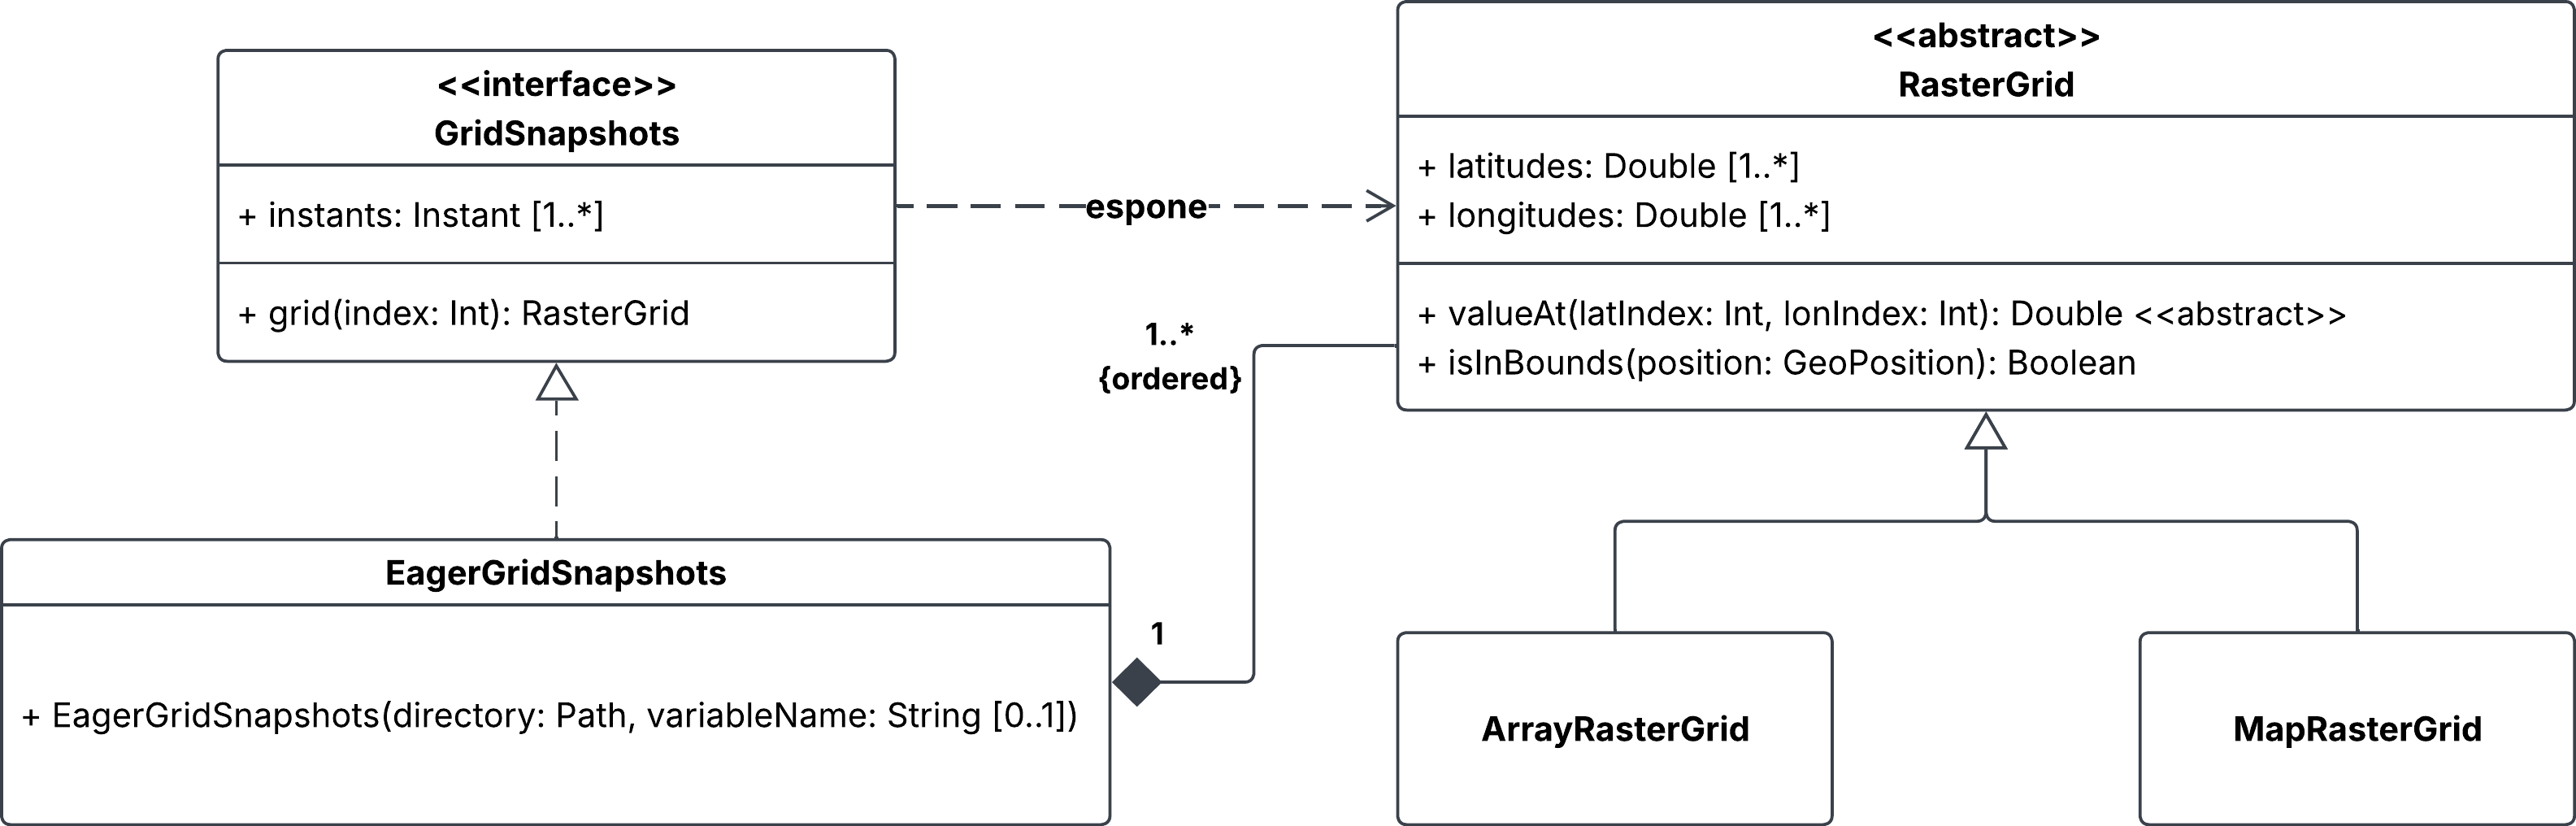
\includegraphics[width=\linewidth]{figures/progettazione/rappresentazione.png}
    \caption[Rappresentazione dei dati raster]{Le astrazioni per una griglia raster e per
    una serie temporale di griglie, con le rispettive realizzazioni.}
    \label{fig:uml-rappresentazione}
\end{figure}

\subsection{La griglia raster}
\label{subsec:raster-grid}

Una griglia raster è definita da due assi indipendenti, di latitudini e di longitudini, e
dai campioni collocati sulle celle che ne risultano. I due assi sono esposti come vettori di
\texttt{Double}; coerentemente con l'ipotesi stabilita nella
Sezione~\ref{subsec:griglie-supportate}, si richiede che siano strettamente monotoni ma non
che siano equispaziati, per cui la posizione di ciascuna coordinata non è ricavabile per via
aritmetica e va conservata esplicitamente. Di conseguenza, l'individuazione della cella che
contiene una data coordinata è una ricerca sull'asse anziché un calcolo.

\texttt{RasterGrid} è una classe astratta e non un'interfaccia. La ragione è che la
validità degli assi, ovvero la loro monotonia stretta, la coerenza fra le loro dimensioni
e il numero dei campioni, è una precondizione che vale per ogni griglia, quale che sia il
modo in cui i campioni siano memorizzati. Collocandone la verifica nel costruttore della
classe astratta, essa viene eseguita per costruzione da ogni realizzazione presente e
futura.

Le due realizzazioni, \texttt{ArrayRasterGrid} e \texttt{MapRasterGrid},
differiscono unicamente nel modo in cui i campioni sono memorizzati, e definiscono
rispettivamente una rappresentazione densa e una sparsa. La distinzione è motivata
dalla variabilità della densità dei dati: una grandezza come la temperatura, campionata
su un'area prevalentemente continentale, riporta una misura in quasi tutte le celle
della griglia; una grandezza come la portata fluviale è invece definita solo lungo i
corsi d'acqua, e lascia priva di misura la maggior parte della griglia.

La scelta fra le due non ricade su chi configura la simulazione: viene effettuata
dinamicamente alla lettura del file, sulla base della densità osservata dei campioni.
Il criterio di scelta è descritto nel Capitolo~\ref{chap:implementazione}.

Si noti che la distinzione è invisibile a chi usa la griglia:
chi vi accede vede unicamente il tipo \texttt{RasterGrid}, e le due realizzazioni
differiscono solo per il compromesso fra memoria occupata e costo di accesso.

\subsection{La serie temporale di griglie}
\label{subsec:grid-snapshots}

\texttt{GridSnapshots} descrive una successione di griglie omogenee, ciascuna associata a
un istante del mondo reale. L'astrazione espone due sole caratteristiche: la successione
ordinata degli istanti e l'accesso alla griglia corrispondente a una data posizione nella
successione. La prima è ciò che consente a chi la interroga di individuare i due istanti
adiacenti a quello richiesto; la seconda, di ottenere le griglie corrispondenti.

La realizzazione fornita, \texttt{EagerGridSnapshots}, costruisce l'intera serie in memoria
al momento della costruzione, leggendo tutti i file presenti in una cartella. La scelta
risponde a \req{NF8}: spostando l'intero accesso al file system nella fase di costruzione,
ogni successiva lettura del layer opera su entità già residenti in memoria, con un costo
indipendente dal formato di origine e dal numero di file da cui la serie è stata ricavata.
La stessa scelta soddisfa \req{NF7}, poiché un file illeggibile o incoerente con gli
altri si manifesta al caricamento della simulazione anziché durante l'esecuzione.

Il prezzo è che l'occupazione di memoria cresce con l'estensione della serie e dell'area
geografica di riferimento. Il vincolo è ritenuto accettabile: le richieste sono formulate
dal modellista in funzione della simulazione che intende condurre. L'astrazione
\texttt{GridSnapshots} non impone comunque questa strategia, e una realizzazione che
carichi le griglie su richiesta è possibile senza alcuna modifica al layer.

Un \ac{GRIB} o \ac{NetCDF} può contenere più variabili distinte: un archivio scaricato da
un data store Copernicus può includere, ad esempio, sia la temperatura a due metri dal suolo
sia la velocità del vento nello stesso file. La costruzione di una serie richiede quindi di specificare
anche quale fra le variabili presenti debba essere estratta. Il nome della variabile può
essere omesso quando i file ne contengono una sola, caso in cui essa è individuata
senza ambiguità.
Il modo in cui una variabile viene individuata ed estratta da un file è discusso nel
Capitolo~\ref{chap:implementazione}. \textbf{\emph{(Capitolo di implementazione)}}

\section{Le strategie di risoluzione dei valori}
\label{sec:risoluzione}

La Sezione~\ref{subsec:discretezza-campioni} ha stabilito, con \req{F5}, che la regola con
cui un valore viene prodotto a partire dai campioni disponibili non può essere fissata nel
codice, ma deve essere configurabile e intercambiabile. Questa sezione ne descrive la
realizzazione come famiglia di strategie, e la estende al secondo passaggio necessario a
produrre il valore restituito dal layer: la traduzione da un \texttt{Double} al tipo
esposto ai nodi, richiesta da \req{F6}.

\subsection{Le strategie di interpolazione}
\label{subsec:interpolazione}

Il requisito si traduce nell'introduzione di un'astrazione per la regola e di
un insieme di realizzazioni intercambiabili, secondo lo schema noto come \emph{strategia}.
La \Cref{fig:uml-interpolazione} riporta la gerarchia risultante.

\begin{figure}[h]
    \centering
    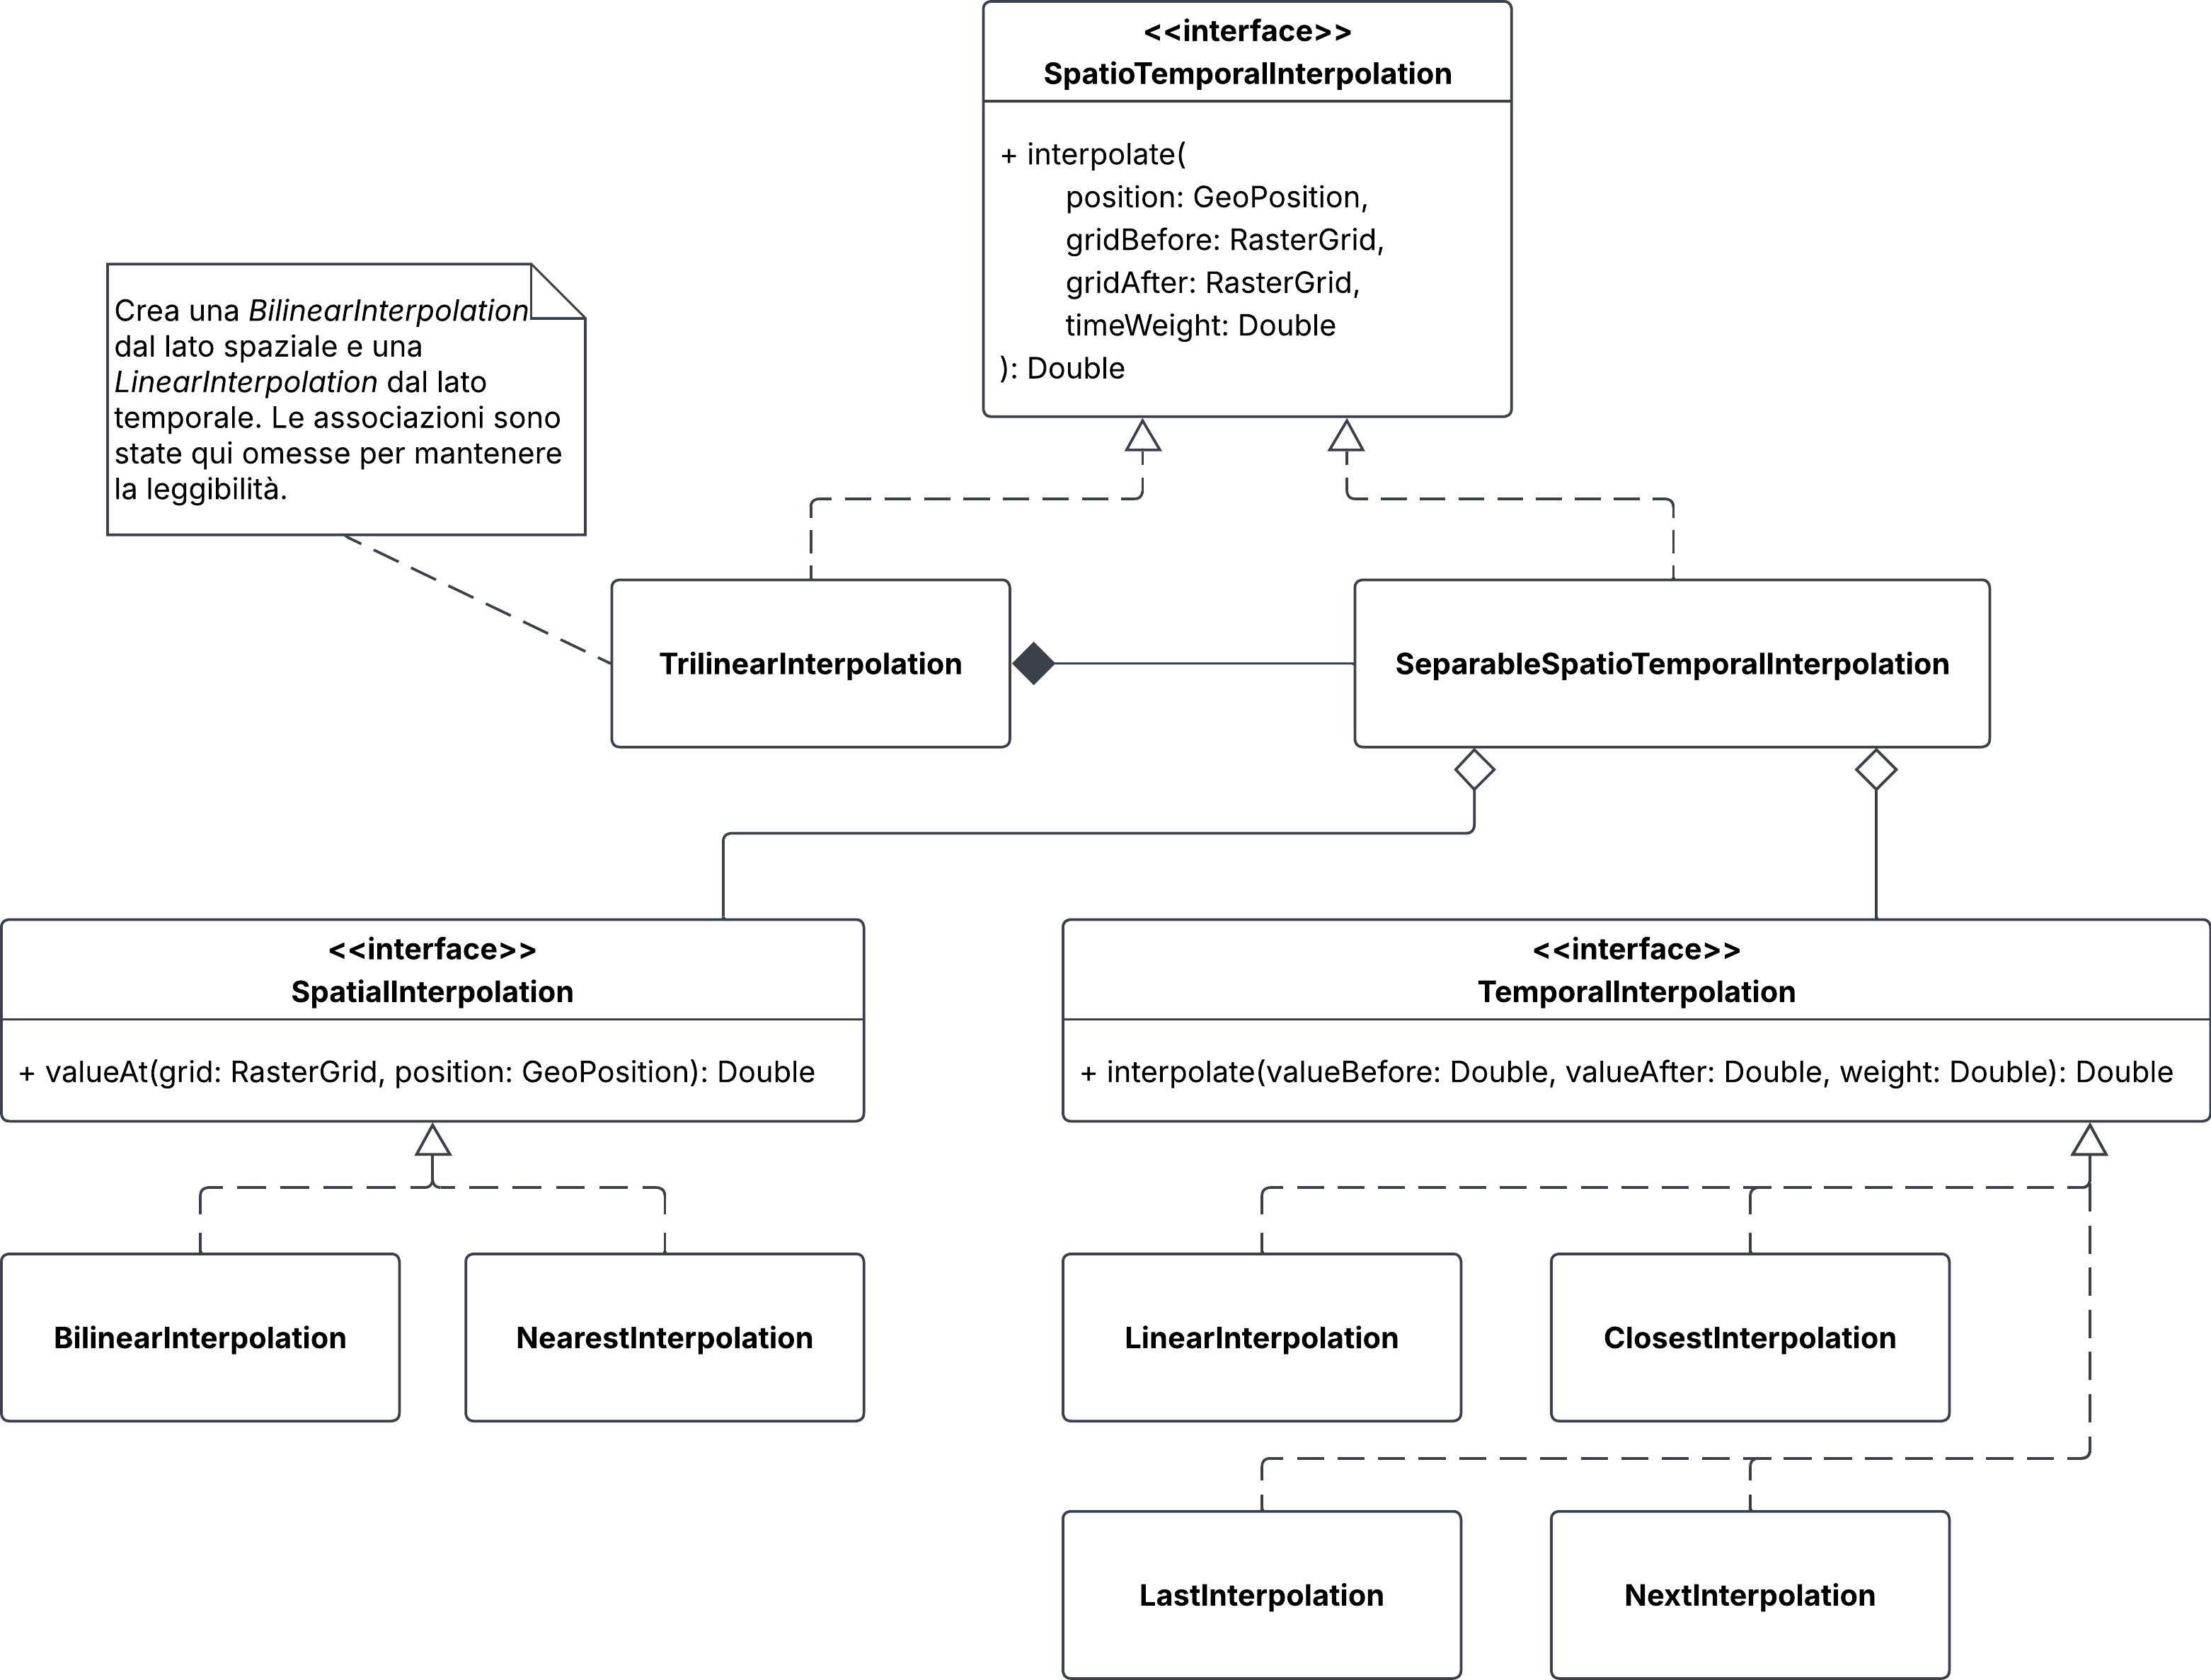
\includegraphics[width=\linewidth]{figures/progettazione/interpolazione.png}
    \caption[Strategie di interpolazione]{Le strategie di interpolazione spaziale,
    temporale e spazio-temporale, e la loro composizione.}
    \label{fig:uml-interpolazione}
\end{figure}

L'astrazione principale, \texttt{SpatioTemporalInterpolation}, attraversa entrambi i
domini: riceve la posizione geografica, due griglie adiacenti all'istante richiesto e
il peso che colloca l'istante richiesto fra i due, e ne produce un valore. La ragione per
cui la regola è espressa da un'unica astrazione anziché da due composte in un ordine
fissato è che non tutte le regole concepibili sono separabili spazialmente e temporalmente: una regola
che consideri contemporaneamente i campioni delle due griglie, senza risolvere prima lo spazio
e poi il tempo, non sarebbe esprimibile.

Altre regole di interesse pratico però sono separabili, ovvero si risolvono collassando
le due griglie spaziali ciascuna a un unico valore in funzione della sola posizione,
per poi decidere il valore finale rispetto alla regola di interpolazione temporale su questi.

Per queste regole, il
modulo introduce \sloppypar{\texttt{SeparableSpatioTemporalInterpolation}}, che realizza l'astrazione
principale componendo due strategie indipendenti: una spaziale, che risolve la posizione
su ciascuna delle due griglie, e una temporale, che combina i due valori così ottenuti
secondo il peso.

Le realizzazioni fornite permettono di distinguere fra grandezze che ammettono valori intermedi e
grandezze che non li ammettono. Sul dominio spaziale, \texttt{BilinearInterpolation}
produce una media pesata dei quattro campioni che circondano la posizione (si veda come riferimento la \Cref{fig:spatial-interp}), adatta a
grandezze continue, mentre \texttt{NearestInterpolation} seleziona il campione della cella
più vicina, scelta ammissibile per grandezze categoriche. Sul dominio temporale,
\texttt{LinearInterpolation} combina i due campioni in proporzione al peso, mentre
\texttt{ClosestInterpolation}, \texttt{LastInterpolation} e \texttt{NextInterpolation} ne
selezionano uno soltanto, rispettivamente il più vicino, il precedente o il successivo.

Fra le combinazioni possibili, una configurazione sufficientemente ricorrente da meritare
un nome proprio, in modo da poter essere istanziata direttamente tramite YAML, è la \texttt{TrilinearInterpolation}.
Essa può essere ottenuta applicando un'interpolazione bilineare sulle due dimensioni spaziali
e una successiva interpolazione lineare lungo quella temporale~\cite{engel2006realtime}.
Quest'ultima non costituisce tuttavia una specializzazione della composizione separabile,
bensì una sua configurazione fissata, e viene quindi realizzata per delegazione.

La strategia di interpolazione è inoltre il punto in cui si decide il destino dei valori
mancanti, qui rappresentati da \texttt{Double.NaN}: \req{F7} ne impone un trattamento
esplicito, e la Sezione~\ref{subsec:discretezza-campioni} ha stabilito che la decisione
dipenda dalla semantica del dato. In \texttt{BilinearInterpolation}, ad esempio, si è
scelto di propagare il valore mancante se almeno uno dei quattro campioni circondanti la
posizione non è presente, e viene allo stesso modo propagato da
\texttt{LinearInterpolation} se uno dei due valori spazialmente risolti è assente.

La verifica che la posizione richiesta ricada entro l'estensione coperta dalle
griglie è compito del layer, e precede l'invocazione della strategia.
Le realizzazioni possono quindi assumere che gli argomenti ricevuti siano ammissibili,
e concentrarsi sulla sola regola di combinazione dei campioni.

\subsection{La conversione del valore}
\label{subsec:conversione}

Risolto il valore numerico, resta il passaggio finale: tradurlo nel tipo esposto dal layer.

\begin{figure}[H]
    \centering
    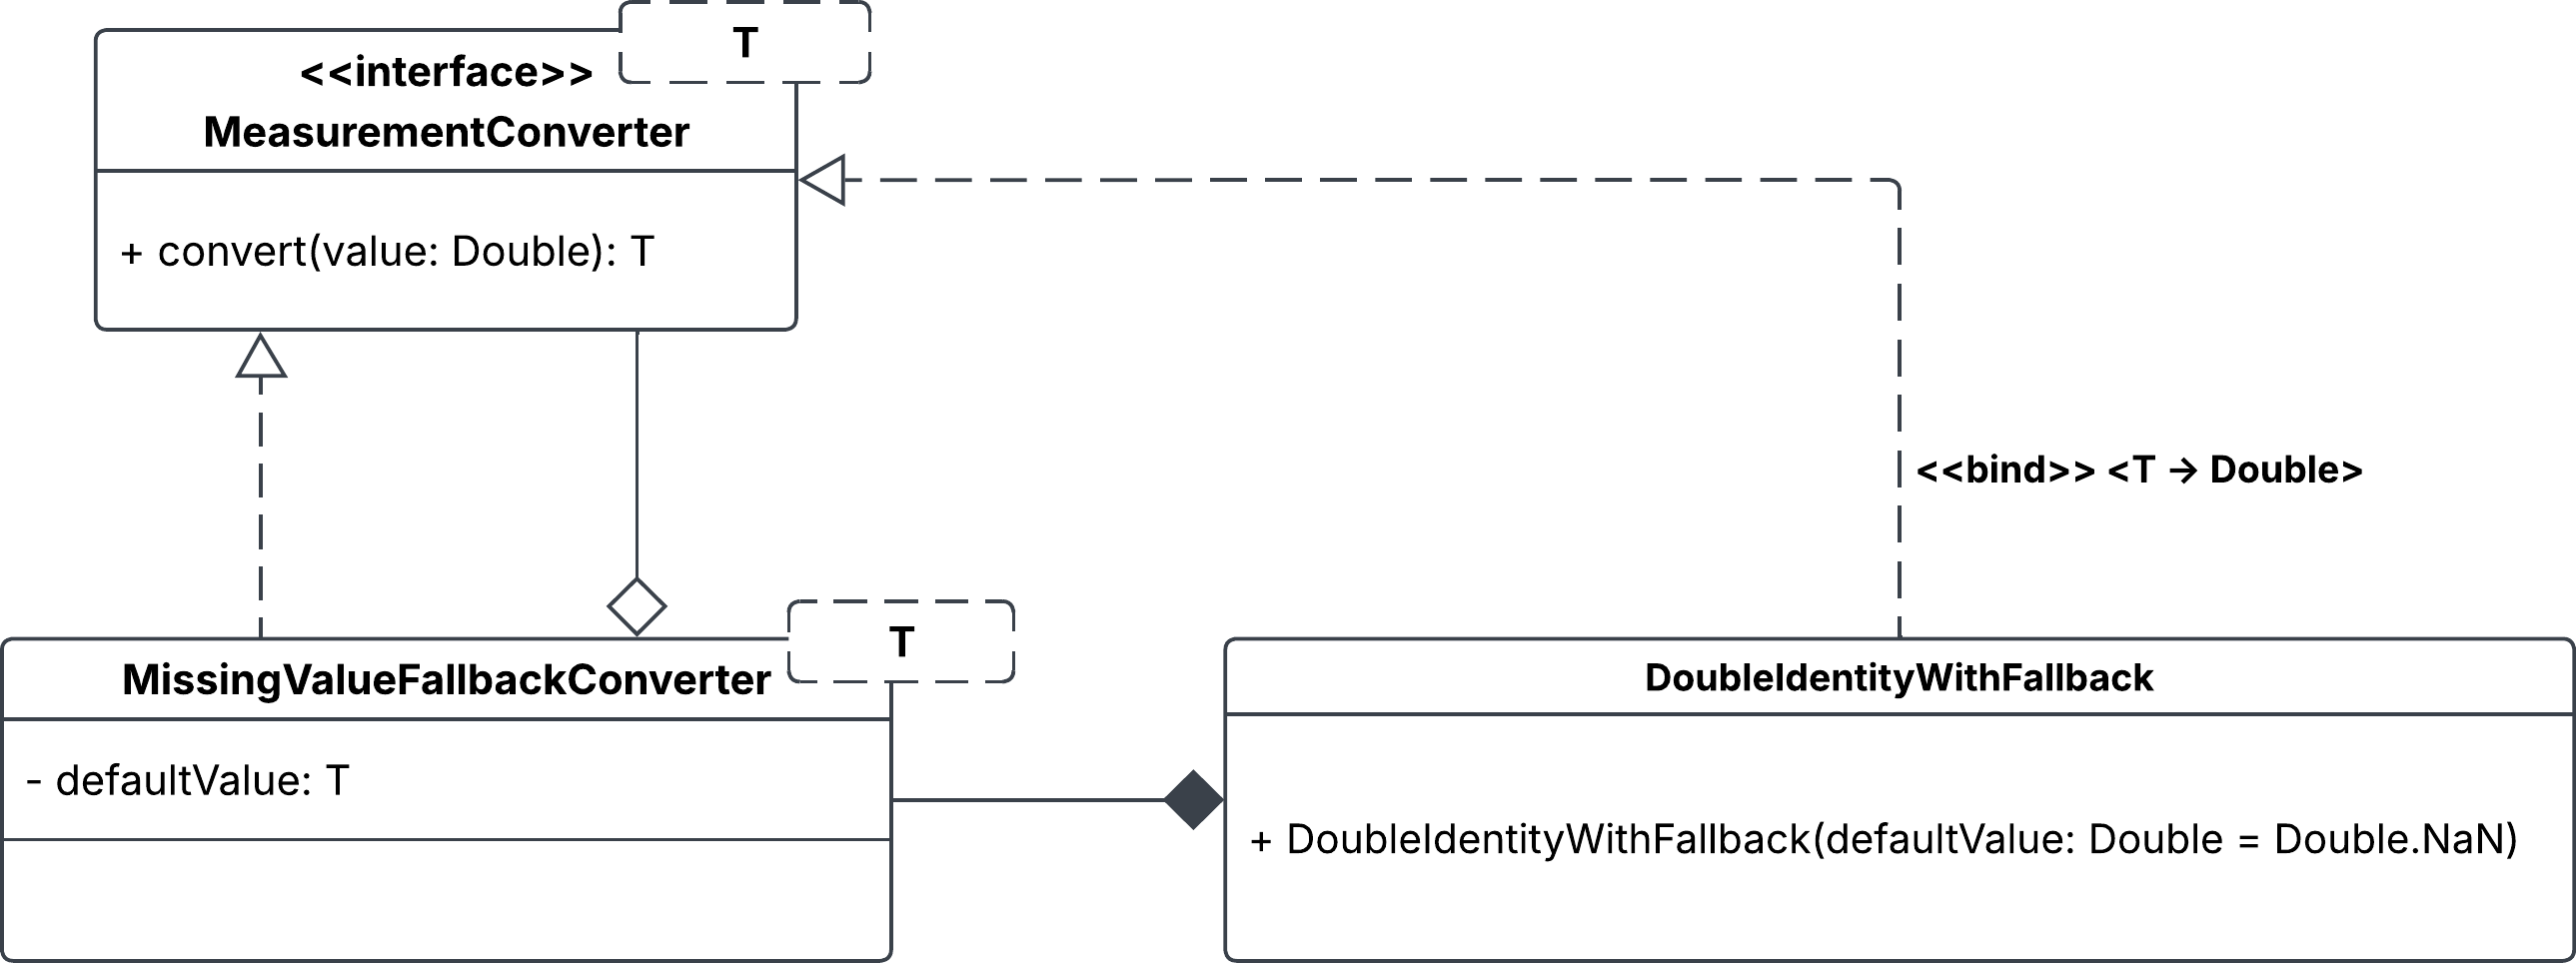
\includegraphics[width=\linewidth]{figures/progettazione/conversione.png}
    \caption[Conversione del valore]{L'astrazione per la conversione del valore risolto e
    la sua composizione con la gestione dei valori mancanti.}
    \label{fig:uml-conversione}
\end{figure}

\texttt{MeasurementConverter<T>} descrive la traduzione da un \texttt{Double} al
tipo \texttt{T} esposto dal layer. È l'unica astrazione del modulo che decide quel tipo,
ed è ciò che soddisfa \req{F6}, consentendo di esporre ai nodi grandezze
la cui interpretazione non è quantitativa, come ad esempio convertendo una soglia in un
valore booleano.

La conversione porta con sé un secondo compito: decidere cosa fare quando il valore
risolto è mancante.
Una scelta che può essere comune nelle simulazioni è poter convertire i valori mancanti
in un valore prefissato, ed è ciò di cui si occupa
\texttt{MissingValueFallbackConverter<T>}, un decoratore che riceve un altro convertitore e un valore di
ripiego: intercetta il caso mancante e restituisce il ripiego, inoltrando ogni altro
valore al convertitore delegato.

\texttt{DoubleIdentityWithFallback} è la configurazione corrispondente al caso più comune,
ovvero un layer che espone direttamente il valore numerico, agendo da funzione identità,
con un possibile ripiego su un valore prestabilito nel caso il dato sia mancante
(propagando il valore assente, se non specificato altrimenti).
Come per \texttt{TrilinearInterpolation}, il suo comportamento viene delegato
poiché è una configurazione fissata a cui si dà un nome, e non una specializzazione della logica.

\section{Il layer Copernicus}
\label{sec:layer}

Il layer è il punto in cui i sottomoduli precedenti vengono composti. La
\Cref{fig:aggr-layer} ne riporta le entità con cui collabora.

\begin{figure}[h]
    \centering
    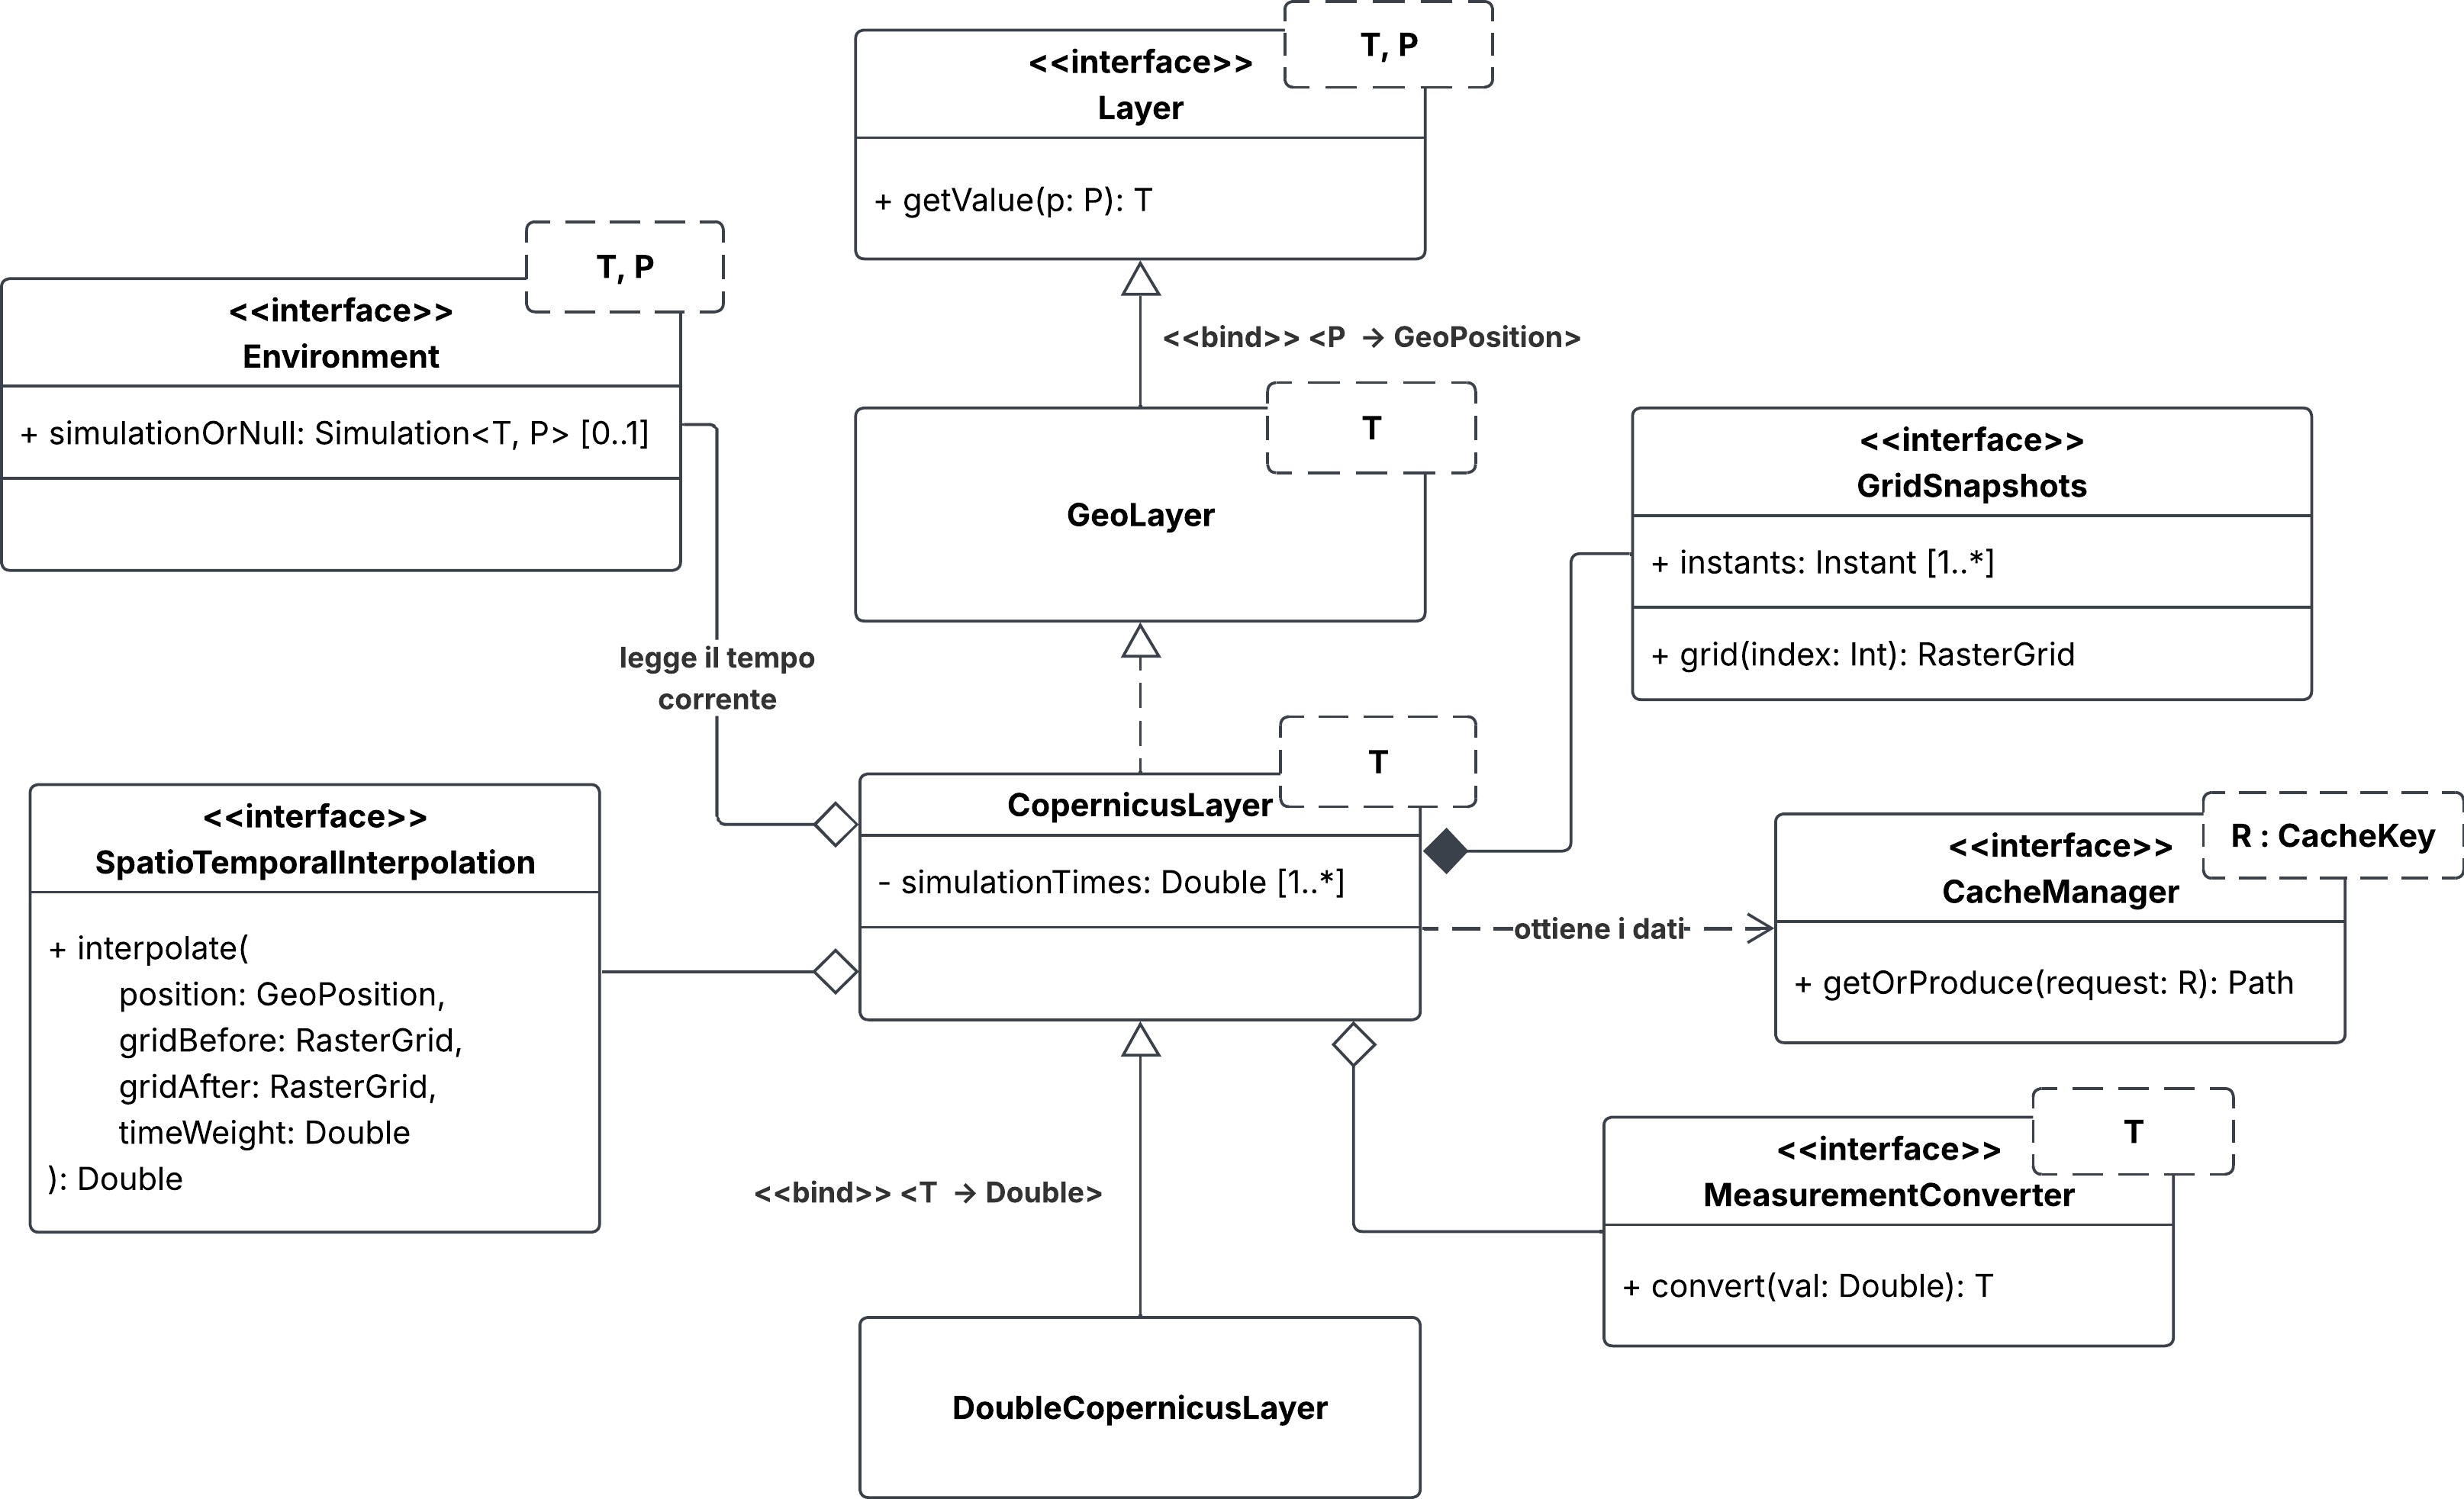
\includegraphics[width=\linewidth]{figures/progettazione/aggr_layer.png}
    \caption[Il layer Copernicus]{La gerarchia del layer e le sue collaborazioni.}
    \label{fig:aggr-layer}
\end{figure}

\subsection{La semantica di interrogazione}
\label{subsec:layer-pull-based}

Il requisito \req{F2} chiede che il valore restituito sia quello percepito all'istante di
simulazione corrente. Perché ciò accada, il layer deve in qualche modo venire a conoscenza
dell'avanzamento del tempo di simulazione, e sono possibili due semantiche opposte.

La prima affida a una reazione dedicata il compito di avanzare esplicitamente lo stato del
layer, in sincronia con l'avanzamento del tempo: a ogni esecuzione, la reazione
aggiornerebbe lo stato corrente esposto dal layer, che si limiterebbe poi a restituirlo.
La seconda non prevede alcuno stato temporale nel layer: quando interrogato, esso legge
autonomamente il tempo di simulazione corrente dall'environment
(Sezione~\ref{subsec:alchemist-time}) e ne ricava il valore.

Il modulo adotta la seconda, per due ragioni:
\begin{itemize}
    \item la prima è di ridondanza: il nodo che interroga il layer vive già
    nell'environment e ne condivide la stessa percezione del tempo, per cui usare una
    reazione dedicata al solo scopo di rendere noto al layer che il tempo è avanzato
    duplicherebbe un'informazione già accessibile al momento della lettura;
    \item la seconda è di determinismo: con una reazione dedicata, il valore letto a un dato
    istante dipenderebbe dall'ordine con cui il motore di simulazione esegue la reazione di
    avanzamento e quella che legge il layer; la semantica a interrogazione elimina il
    problema alla radice, non essendoci alcuno stato da sincronizzare.
\end{itemize}

Per le stesse ragioni, il progetto non introduce un'interfaccia dedicata che aggiunga il
concetto di layer temporale: un layer per dati Copernicus è un'implementazione di
\texttt{Layer<T, GeoPosition>} come un'altra, e non un tipo concettualmente distinto.

\iffalse
\subsection{La corrispondenza temporale}
\label{subsec:layer-corrispondenza}

Letto il tempo di simulazione corrente, il layer deve stabilire a quale istante del mondo
reale esso corrisponda. La Sezione~\ref{subsec:corrispondenza-temporale} ha stabilito che
tale corrispondenza vada confinata nel solo componente che ne ha bisogno, ed è quindi il
layer a ospitarla.

La corrispondenza è definita da due soli parametri: un'\emph{origine}, l'istante reale a
cui corrisponde lo zero del tempo di simulazione, e una \emph{scala}, la durata reale
rappresentata da un'unità di tempo simulato. Fissati questi due valori, ogni istante di
simulazione individua un istante reale e viceversa. Entrambi sono dichiarati da chi
configura la simulazione, come \req{F3} richiede, e restano costanti per l'intera
esecuzione.

L'origine ammette un valore predefinito, ovvero il primo istante coperto dalla
serie, che corrisponde al caso più frequente di una simulazione che inizia
con i dati di cui dispone.

La corrispondenza è stabilita una sola volta, al momento della costruzione del layer, e non
è nota ad alcun'altra parte del simulatore, che continua a operare su un tempo scalare. Ne
consegue che le modifiche richieste da un'eventuale futura migrazione del tipo di tempo di
Alchemist resterebbero circoscritte a un unico punto del modulo.

Ottenuto l'istante reale, resta il caso in cui esso ricada al di fuori dell'intervallo
coperto dalla serie, che la Sezione~\ref{subsec:estensione-spaziale} ha stabilito non
costituire un errore di modellazione. Il layer estrapola a valore costante: se l'istante
precede il primo disponibile viene considerato quest'ultimo, e analogamente, se supera
l'ultimo, viene considerato l'ultimo istante presente nei dati.
\fi
\subsection{La corrispondenza temporale}
\label{sec:corrispondenza-temporale}

Il layer deve mettere in relazione due domini temporali di natura diversa: il tempo
di simulazione, che legge dall'environment quando viene interrogato, e gli istanti
del mondo reale a cui sono riferite le griglie della serie che espone. La
Sezione~\ref{subsec:corrispondenza-temporale} ha stabilito che tale corrispondenza vada
confinata nel solo componente che ne ha bisogno, ed è quindi il layer a ospitarla.

La corrispondenza è definita da due soli parametri: un'\emph{origine}, l'istante
reale a cui corrisponde lo zero del tempo di simulazione, e una \emph{scala}, la
durata reale rappresentata da un'unità di tempo simulato. Fissati questi due valori,
ogni istante di simulazione individua un istante reale e viceversa. Entrambi sono
dichiarati da chi configura la simulazione, come \req{F3} richiede, e restano
costanti per l'intera esecuzione. L'origine ammette un valore predefinito, il primo
istante coperto dalla serie, che corrisponde al caso più frequente di una
simulazione che inizia con i dati di cui dispone.

Essendo la corrispondenza biunivoca, essa può essere applicata in due
direzioni opposte: tradurre a ogni interrogazione il tempo di simulazione corrente
nell'istante reale che gli corrisponde, oppure tradurre una volta sola l'intera
successione degli istanti della serie in tempi di simulazione. Il modulo adotta la
seconda: alla costruzione del layer l'asse temporale della serie viene ricondotto al
tempo di simulazione, e il layer conserva la successione così ottenuta in un
vettore di scalari.

La scelta fa della costruzione l'unico punto in cui i due domini si incontrano.
Tutto ciò che avviene durante l'esecuzione, ovvero l'individuazione dei due campioni
che racchiudono l'istante richiesto, il calcolo del peso temporale e il trattamento
degli istanti esterni all'intervallo coperto, opera tramite
il valore letto dall'environment.

La conversione è ospitata dal layer e non dalla serie di griglie. Questo perché
\texttt{GridSnapshots} descrive dati, non una simulazione, e i suoi istanti
restano quelli del mondo reale a cui le griglie sono riferite, indipendentemente da
quale simulazione li utilizzi e con quale convenzione.

Resta il caso in cui il tempo di simulazione corrente ricada al di fuori
dell'intervallo coperto dall'asse così ottenuto, che la
Sezione~\ref{subsec:estensione-spaziale} ha stabilito non costituire un errore di
modellazione. Il layer estrapola a valore costante: se l'istante richiesto precede
il primo disponibile viene considerato quest'ultimo e, analogamente, se supera
l'ultimo viene considerato l'ultimo presente nei dati.

Poiché la corrispondenza è stabilita una sola volta, alla costruzione, e non è nota
ad alcun'altra parte del simulatore, che continua a operare su un tempo scalare, le
modifiche richieste da un'eventuale futura migrazione del tipo di tempo di Alchemist
resterebbero circoscritte a un unico punto del modulo.

\subsection{Collocazione nella gerarchia e responsabilità}
\label{subsec:layer-gerarchia}

Fra l'interfaccia \texttt{Layer<T, P>} di Alchemist e la realizzazione concreta è
interposta \texttt{GeoLayer<T>}, che fissa il tipo delle posizioni a \texttt{GeoPosition}
lasciando libero il tipo del valore esposto. L'astrazione intermedia non aggiunge alcun
metodo: il suo scopo è dare un nome alla specializzazione geospaziale del layer.

\texttt{CopernicusLayer<T>} realizza tale astrazione, e le sue responsabilità sono tutte di
coordinamento: individuare le griglie pertinenti al momento in cui viene interrogato e
delegare alle strategie la produzione del valore. Il layer non contiene alcuna logica di
interpolazione né alcuna conoscenza dei formati di origine: è il luogo in cui le decisioni
prese altrove vengono applicate nell'ordine corretto.

La \Cref{fig:layer-sequenza} riporta la distribuzione delle responsabilità fra il layer e 
le entità con cui interagisce nel corso di una singola interrogazione.

\begin{figure}[H]
    \centering
    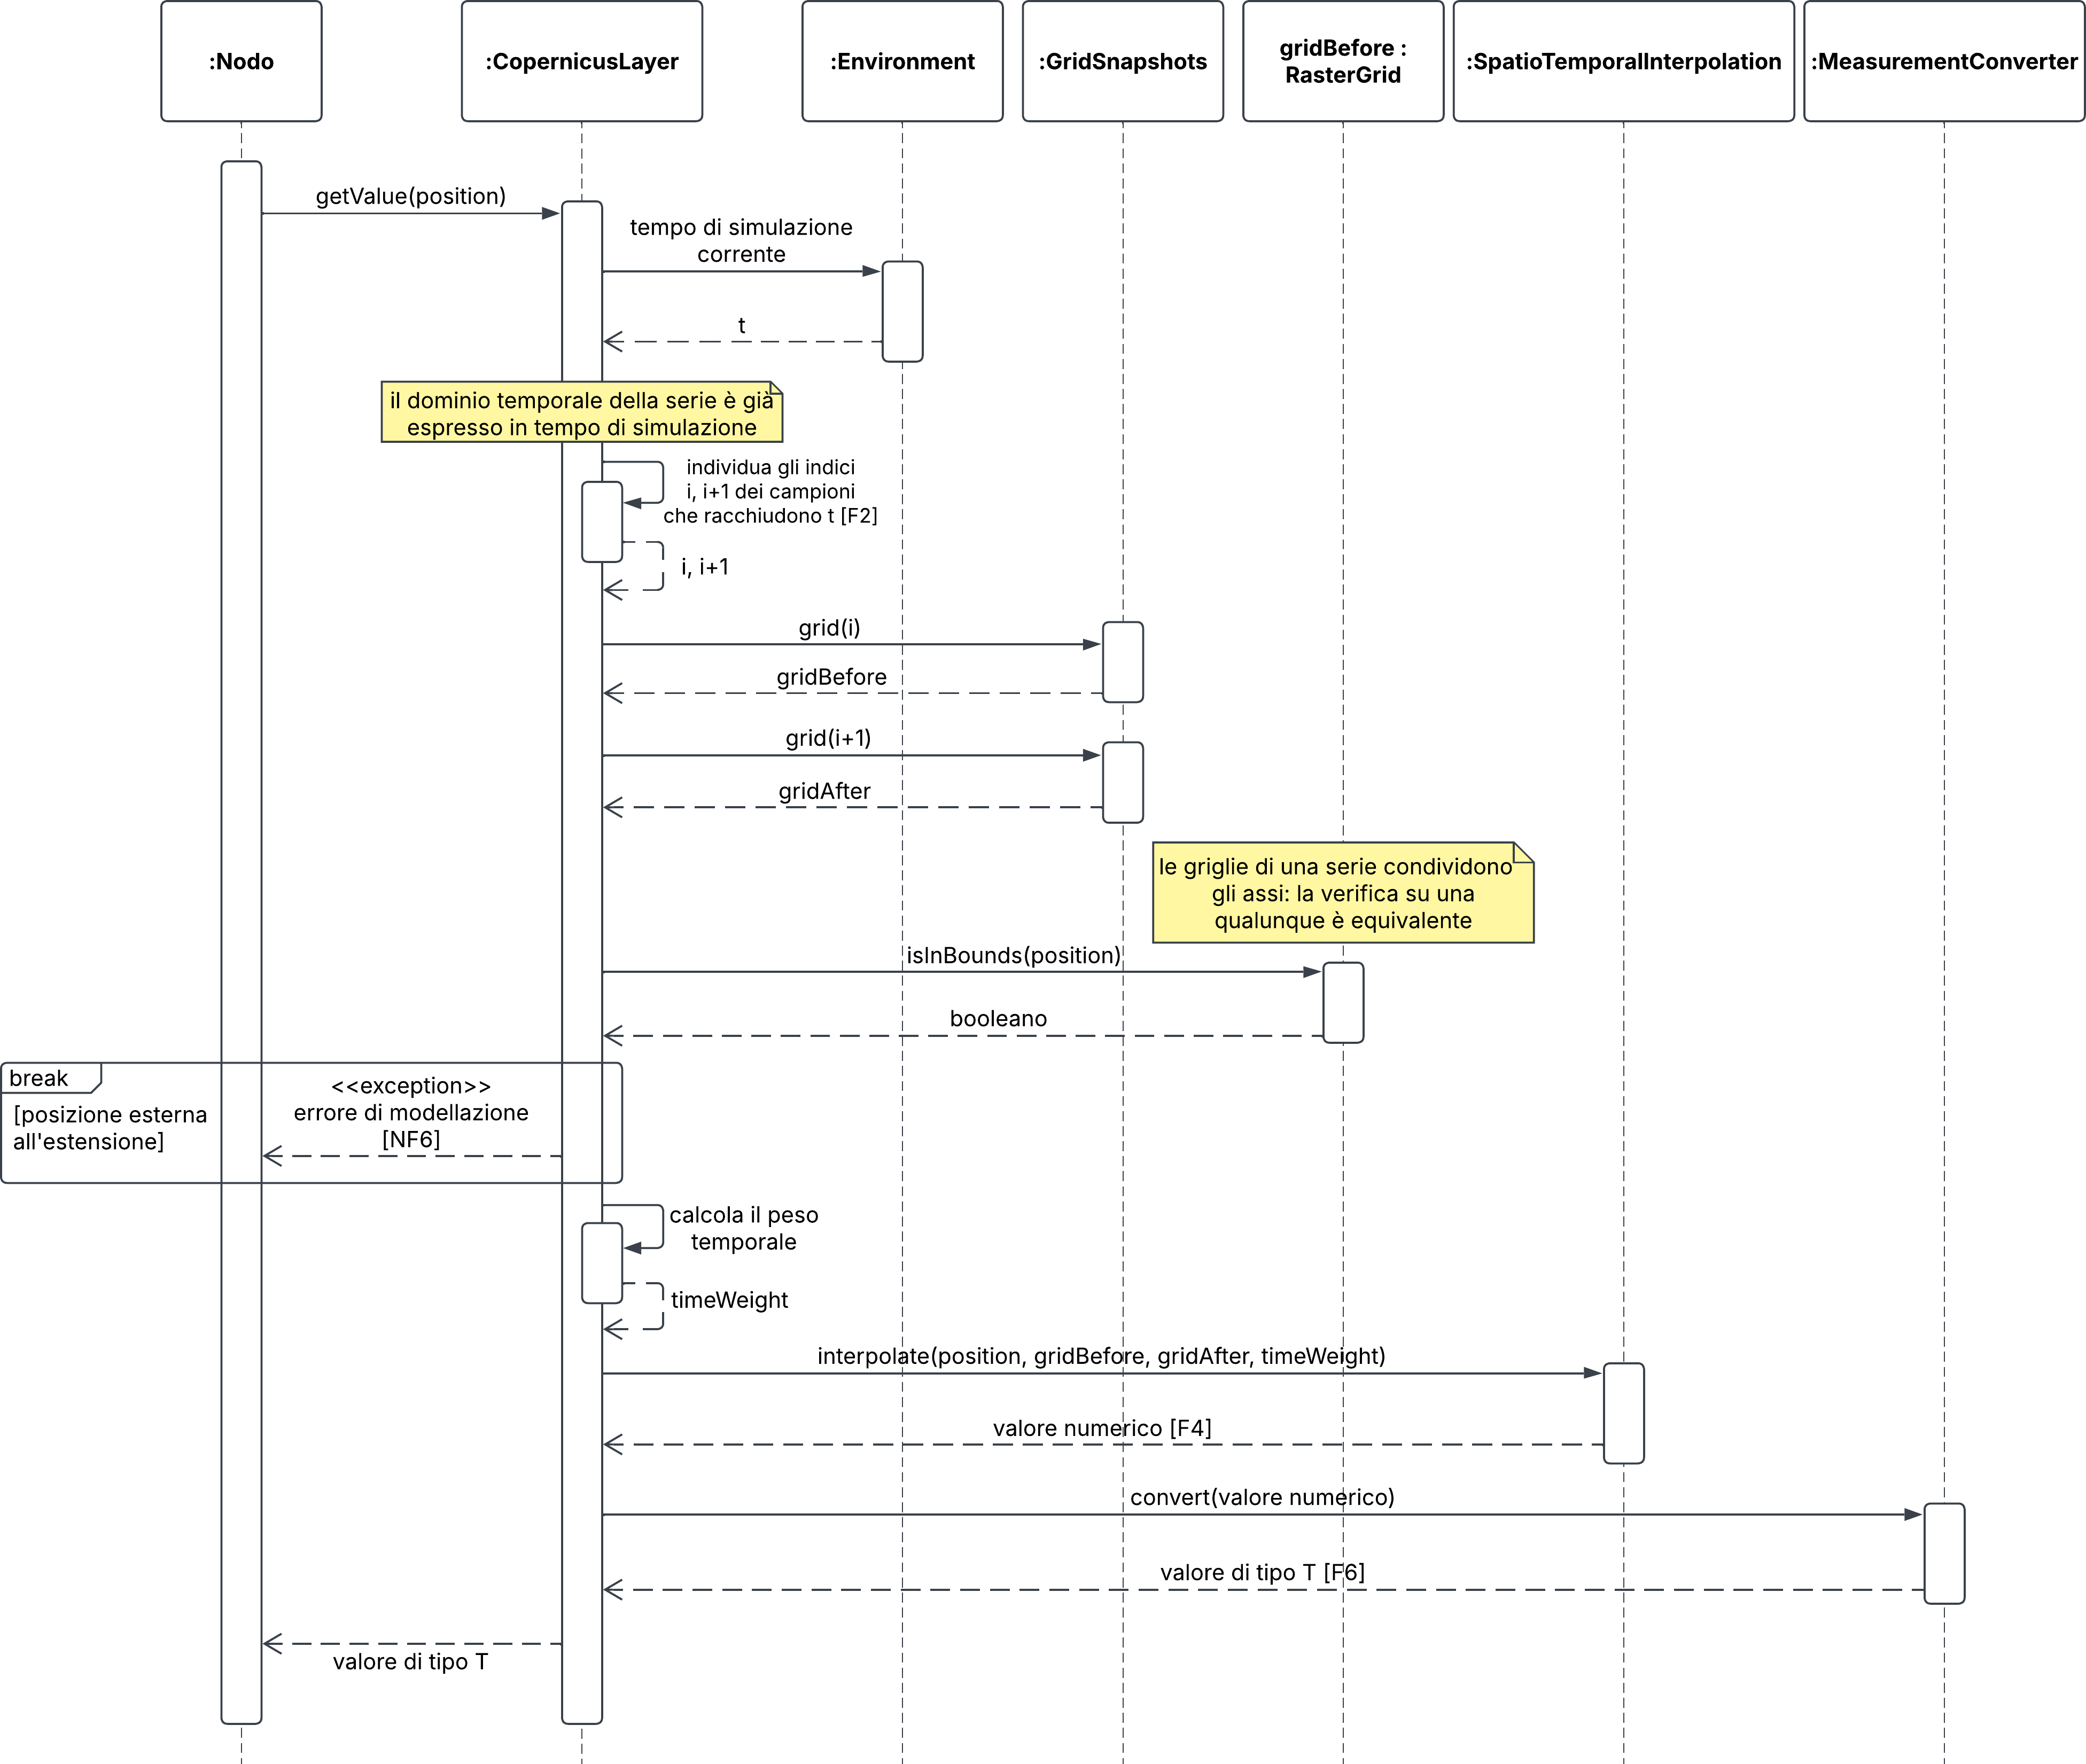
\includegraphics[width=\linewidth]{figures/progettazione/sequenza_layer.png}
    \caption[Interrogazione del layer]{Le interazioni fra il layer e le entità con cui collabora quando gli viene richiesto un valore.}
    \label{fig:layer-sequenza}
\end{figure}

La lettura del tempo di simulazione dall'environment attua la semantica discussa nella
Sezione~\ref{subsec:layer-pull-based}: è il layer a procurarselo al momento
dell'interrogazione, e non un evento esterno a comunicarglielo. L'istante così ottenuto
viene ricondotto al dominio temporale dei dati secondo la corrispondenza fissata alla
costruzione, individuando i due campioni
temporali che lo racchiudono e, con essi, le griglie corrispondenti (\req{F3}).

Disponendo delle griglie, il layer può verificare che la posizione richiesta ricada nella
regione da esse coperta. La verifica attua la delimitazione stabilita nella
Sezione~\ref{subsec:estensione-spaziale}: una posizione esterna non individua alcuna
misura, e la richiesta viene respinta anziché produrre un valore plausibile ma infondato
(\req{NF6}).

Superata la verifica, il layer calcola il peso temporale, che esprime la posizione relativa
dell'istante richiesto fra le due griglie nella forma attesa dalla strategia di
interpolazione.

Le due deleghe finali affidano a componenti esterni al layer le decisioni che dipendono
dalla semantica della grandezza esposta: la produzione del valore numerico a partire dai
campioni adiacenti (\req{F4}) e la sua traduzione nel tipo esposto ai nodi (\req{F6}).

Nessuno di questi passi accede a risorse esterne, come \req{NF8} richiede: la serie di
griglie è già residente in memoria, e la corrispondenza temporale è stata fissata alla
costruzione.

\subsection{Le modalità di costruzione}
\label{subsec:layer-costruzione}

Il layer prevede tre modalità di costruzione, ordinate per ampiezza decrescente di ciò che
si assume già disponibile.

\begin{enumerate}
    \item \textbf{Da una serie già disponibile}: il layer riceve direttamente una
    \texttt{GridSnapshots}, senza sapere da dove provenga.
    \item \textbf{Da una cartella locale}: il layer riceve la collocazione di una cartella
    contenente file già presenti sulla macchina, e da essi costruisce la serie.
    \item \textbf{Da un data store remoto}: il layer riceve la descrizione di una richiesta verso un
    data store Copernicus, e ne ottiene una cartella tramite il sottosistema di
    acquisizione (Sezione~\ref{sec:acquisizione}).
\end{enumerate}

Le tre modalità sono stratificate: ciascuna produce l'argomento della precedente,
riducendosi così alla prima. Poiché ciò che le distingue riguarda
esclusivamente il modo in cui la serie viene ottenuta, e non ciò che il layer ne
fa una volta ottenuta, il comportamento del layer è verificabile in isolamento
fornendo direttamente una serie, senza leggere file né accedere alla rete, come
\req{NF4} richiede.

L'ipotesi stabilita nella Sezione~\ref{subsec:griglie-supportate} riguarda la forma della griglia,
ma non la provenienza dei file. Un dataset campionato su una griglia in proiezione
cartografica non è utilizzabile nella forma in cui il data store lo distribuisce,
ma lo diventa una volta ricondotto a una griglia definita da assi indipendenti di
latitudine e longitudine. La costruzione a partire da una cartella locale accoglie anche
questo caso: il file convertito viene letto come qualunque altro.

In tutte e tre le modalità, inoltre, l'acquisizione e la lettura dei dati
avvengono per intero durante la costruzione del layer, ovvero al caricamento
della simulazione: è quindi lì che si manifesta ogni condizione che impedisca
alla simulazione di disporre dei dati di cui ha bisogno, come \req{NF7} richiede. 

La classe \texttt{CopernicusLayer<T>} è generica nel tipo esposto; il modulo fornisce anche
\texttt{DoubleCopernicusLayer}, che ne fissa il parametro al tipo numerico. La sua
esistenza soddisfa \req{F11}: il meccanismo di caricamento delle simulazioni non è in
grado di istanziare una classe generica, mentre può farlo con una sua specializzazione
concreta (Sezione~\ref{subsec:alchemist-loader}). La specializzazione è inoltre il punto in cui i valori predefiniti delle
strategie possono essere stabiliti, cosa non possibile nella classe generica, non essendo
definibile un convertitore predefinito verso un tipo arbitrario.

Il modo in cui vengono definiti i tre costruttori e i valori di default dei loro
argomenti sono discussi nel Capitolo~\ref{chap:implementazione}. \textbf{\emph{(Capitolo di implementazione)}}

\section{Il sottosistema di acquisizione dati}
\label{sec:acquisizione}

L'ultimo sottomodulo risponde al sotto-problema di acquisizione: ottenere i dati da un
servizio remoto in modo riproducibile, senza riscaricarli a ogni esecuzione
(\req{F9}, \req{F10}). La \Cref{fig:uml-acquisizione} ne riporta le astrazioni e le
realizzazioni.

\begin{figure}[H]
    \centering
    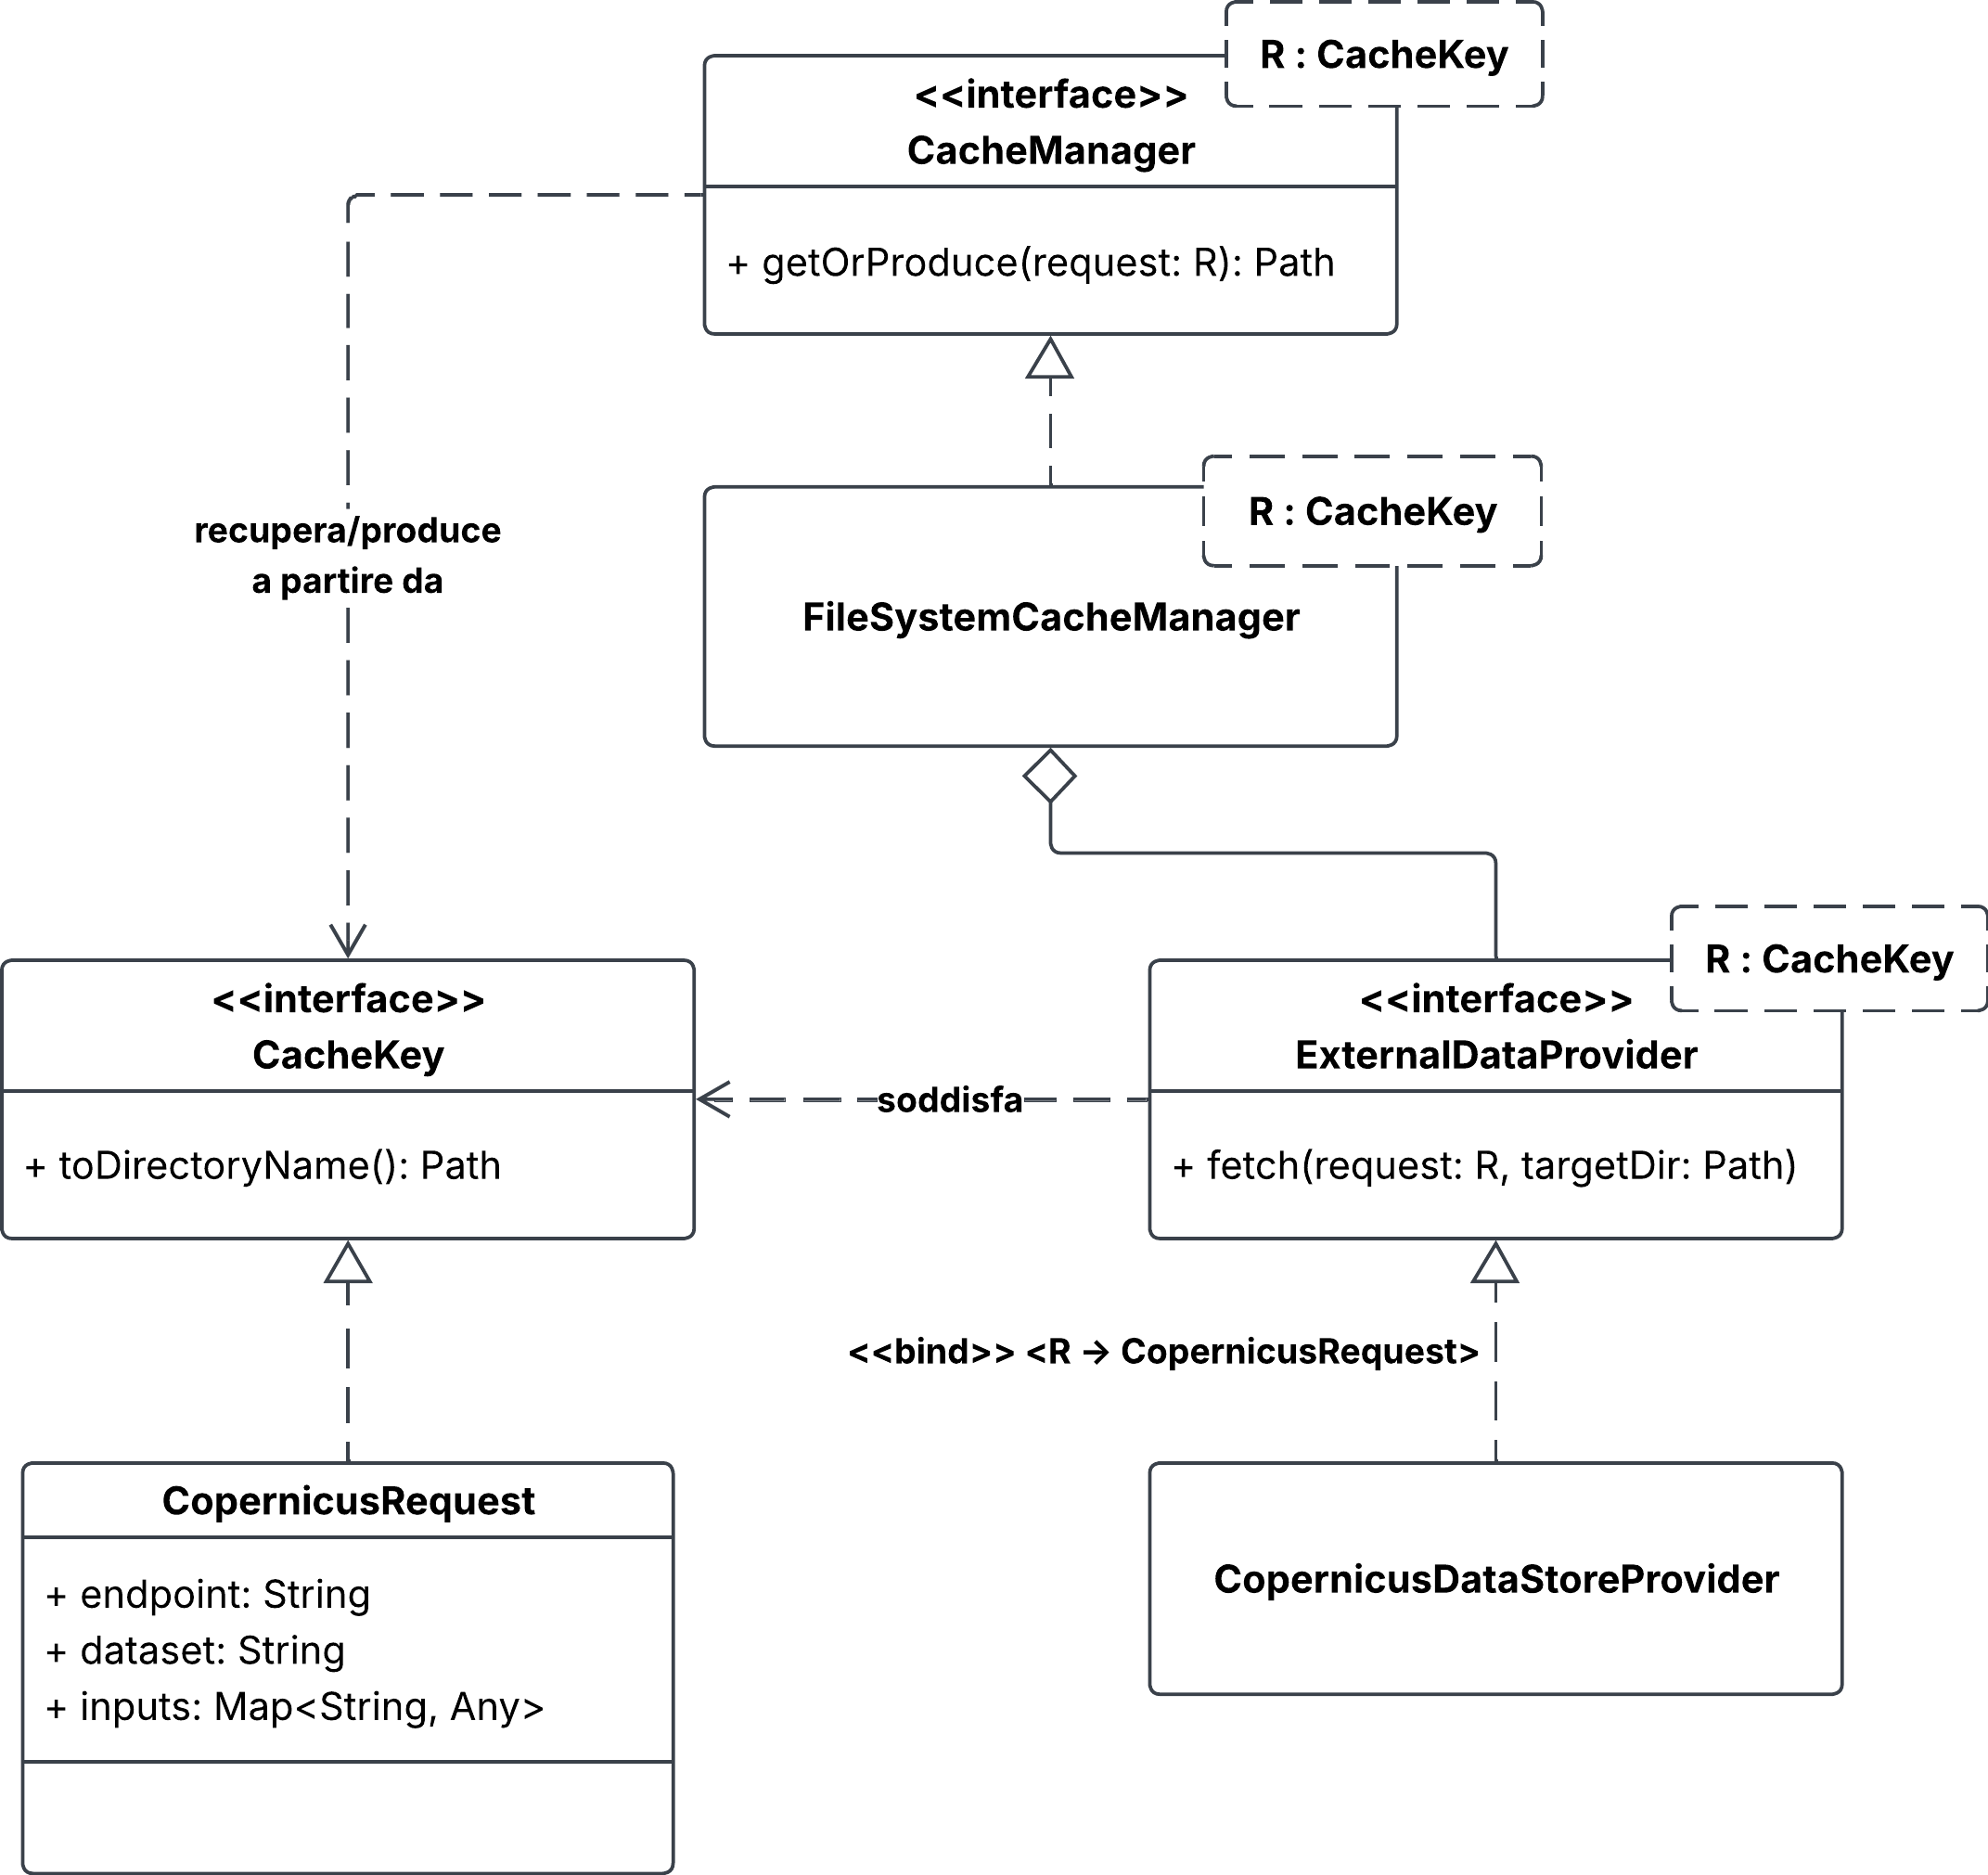
\includegraphics[width=0.9\linewidth]{figures/progettazione/acquisizione.png}
    \caption[Il sottosistema di acquisizione]{Le astrazioni per la cache e per l'accesso a
    fonti esterne, e le realizzazioni relative ai data store Copernicus.}
    \label{fig:uml-acquisizione}
\end{figure}

\subsection{Le astrazioni}
\label{subsec:acquisizione-astrazioni}

Il sottosistema è costruito su tre astrazioni, corrispondenti alle entità individuate nel
modello del dominio:

\begin{itemize}
    \item \texttt{CacheKey}: la descrizione dei dati da ottenere, che ne costituisce
    l'identità. L'unica capacità che l'astrazione richiede è di sapersi tradurre in un nome
    di cartella deterministicamente, in modo tale che descrizioni uguali producano lo stesso nome e
    descrizioni diverse nomi diversi.
    \item \texttt{ExternalDataProvider<R>}: la fonte in grado di soddisfare una
    descrizione, depositando i file corrispondenti in una cartella indicata dal chiamante.
    L'astrazione non indica né il modo né il formato: si limita a stabilire che,
    al termine dell'operazione, la cartella contenga i dati richiesti.
    \item \texttt{CacheManager<R>}: l'entità che, data una descrizione, restituisce la
    cartella contenente i dati corrispondenti, interpellando la fonte esterna solo quando
    non siano già disponibili localmente.
\end{itemize}

Tutte e tre sono parametriche nel tipo della descrizione, vincolato a essere una
\texttt{CacheKey}. Il parametro è ciò che garantisce staticamente che un
gestore di cache e la fonte a cui esso si rivolge accettino la stessa descrizione, senza
che tale coerenza debba essere verificata a tempo di esecuzione.

\subsection{L'indipendenza dalla fonte}
\label{subsec:acquisizione-indipendenza}

Il gestore della cache, \texttt{FileSystemCacheManager<R>}, è indipendente dalla natura della
fonte. Il suo compito consiste nel risolvere il nome della cartella a partire dalla
descrizione, verificarne l'esistenza, e in caso contrario invocare la fonte e conservarne
il risultato nel file system: nessuna di queste operazioni richiede di sapere se i dati
provengano da un data store Copernicus, da un servizio di estrazione cartografica o da
qualunque altra sorgente. Le uniche realizzazioni che conoscono i data store Copernicus
sono \texttt{CopernicusRequest}, che descrive una richiesta verso di essi, e
\texttt{CopernicusDataStoreProvider}, che la soddisfa dialogando con il servizio remoto
secondo il paradigma descritto nella Sezione~\ref{sec:ogc-api-processes}.

È questa suddivisione a rendere effettivo \req{NF2}. In questo modo il sistema
di acquisizione può essere facilmente esteso per supportare altre fonti di dati;
ad esempio, per il recupero
di estratti cartografici da OpenStreetMap, necessario a popolare un
\texttt{OSMEnvironment} (Sezione~\ref{subsec:alchemist-osm}): un servizio di questo tipo
non condivide con i data store Copernicus né il formato dei dati consegnati né il
protocollo con cui la richiesta viene formulata.
Estendere il sottosistema per accoglierlo richiederebbe tuttavia di
realizzare soltanto la coppia \texttt{CacheKey} ed \texttt{ExternalDataProvider<R>}
corrispondente, senza modificare né il gestore della cache né alcuna delle parti già
descritte.

Come il gestore della cache riesce a soddisfare il requisito \req{NF9} è descritto
nel Capitolo~\ref{chap:implementazione}. \textbf{\emph{(Capitolo di implementazione)}}

\subsection{L'identità di una richiesta}
\label{subsec:acquisizione-identita}

Il requisito \req{NF5} chiede che la stessa richiesta corrisponda in modo deterministico
alla stessa voce di cache, ed è ciò che rende possibile \req{F10}. Ciò richiede di
stabilire che cosa costituisca l'identità di una richiesta verso un data store Copernicus,
e come tale identità venga tradotta in un nome di cartella.

L'identità è data dalla terna costituita dal data store interrogato, dal dataset richiesto
e dalla selezione dei parametri con cui la richiesta è stata formulata. Quest'ultima è
deliberatamente non tipizzata: come osservato nella Sezione~\ref{sec:copernicus}, i tre
data store condividono la stessa infrastruttura ma non il catalogo, e ogni dataset ammette
una selezione di parametri propria; imporre una struttura fissa avrebbe limitato
il modulo all'utilizzo di pochi dataset, in contrasto con \req{F8}.

Nel Capitolo~\ref{chap:implementazione} viene discusso come la selezione dei parametri
viene rappresentata e il modo in cui l'identità della richiesta viene tradotta
deterministicamente nel nome di una cartella in cache.